\subsection{Adding External Knowledge}
\label{sec:wiki}

% All of the wikipedia inclusion work.

Motivated by the intuition that phrases gain importance because of both their role in a document and their semantic meaning in the broader world, we experimented with multiple algorithms that incorporate outside knowledge. Each algorithm integrates Wikipedia as a knowledge source in different ways.

\subsubsection{Boosting Documents}

The first algorithm attaches each lecture with a closely related Wikipedia page, and then uses the previously described statistical and linguistic techniques to choose keywords from the combined document. Formally, the procedure is as follows. First, for each lecture, the algorithm takes the title of the lecture, removes stopwords, and uses the result as a query to Wikipedia. Then, the best Wikipedia page match is concatenated to the lecture transcript. After attaching a Wikipedia page to each transcript, we run the previously described procedures over the collection of concatenated lectures and Wikipedia pages.

For example, for the lecture titled ``View Modifications Using Triggers'', the Wikipedia query will return the Wikipedia page titled ``Database trigger'', which is then concatenated to the transcript from the lecture. Then, using either n-grams or adjective-noun phrases as candidate keywords, the algorithm chooses keywords with TF-IDF over the combined document.

\begin{figure}[h!]
\caption{The Document Boosting algorithm searches for a Wikipedia page using the title of the lecture, concatenates the result to the lecture, and then runs TF-IDF over the combined document.}
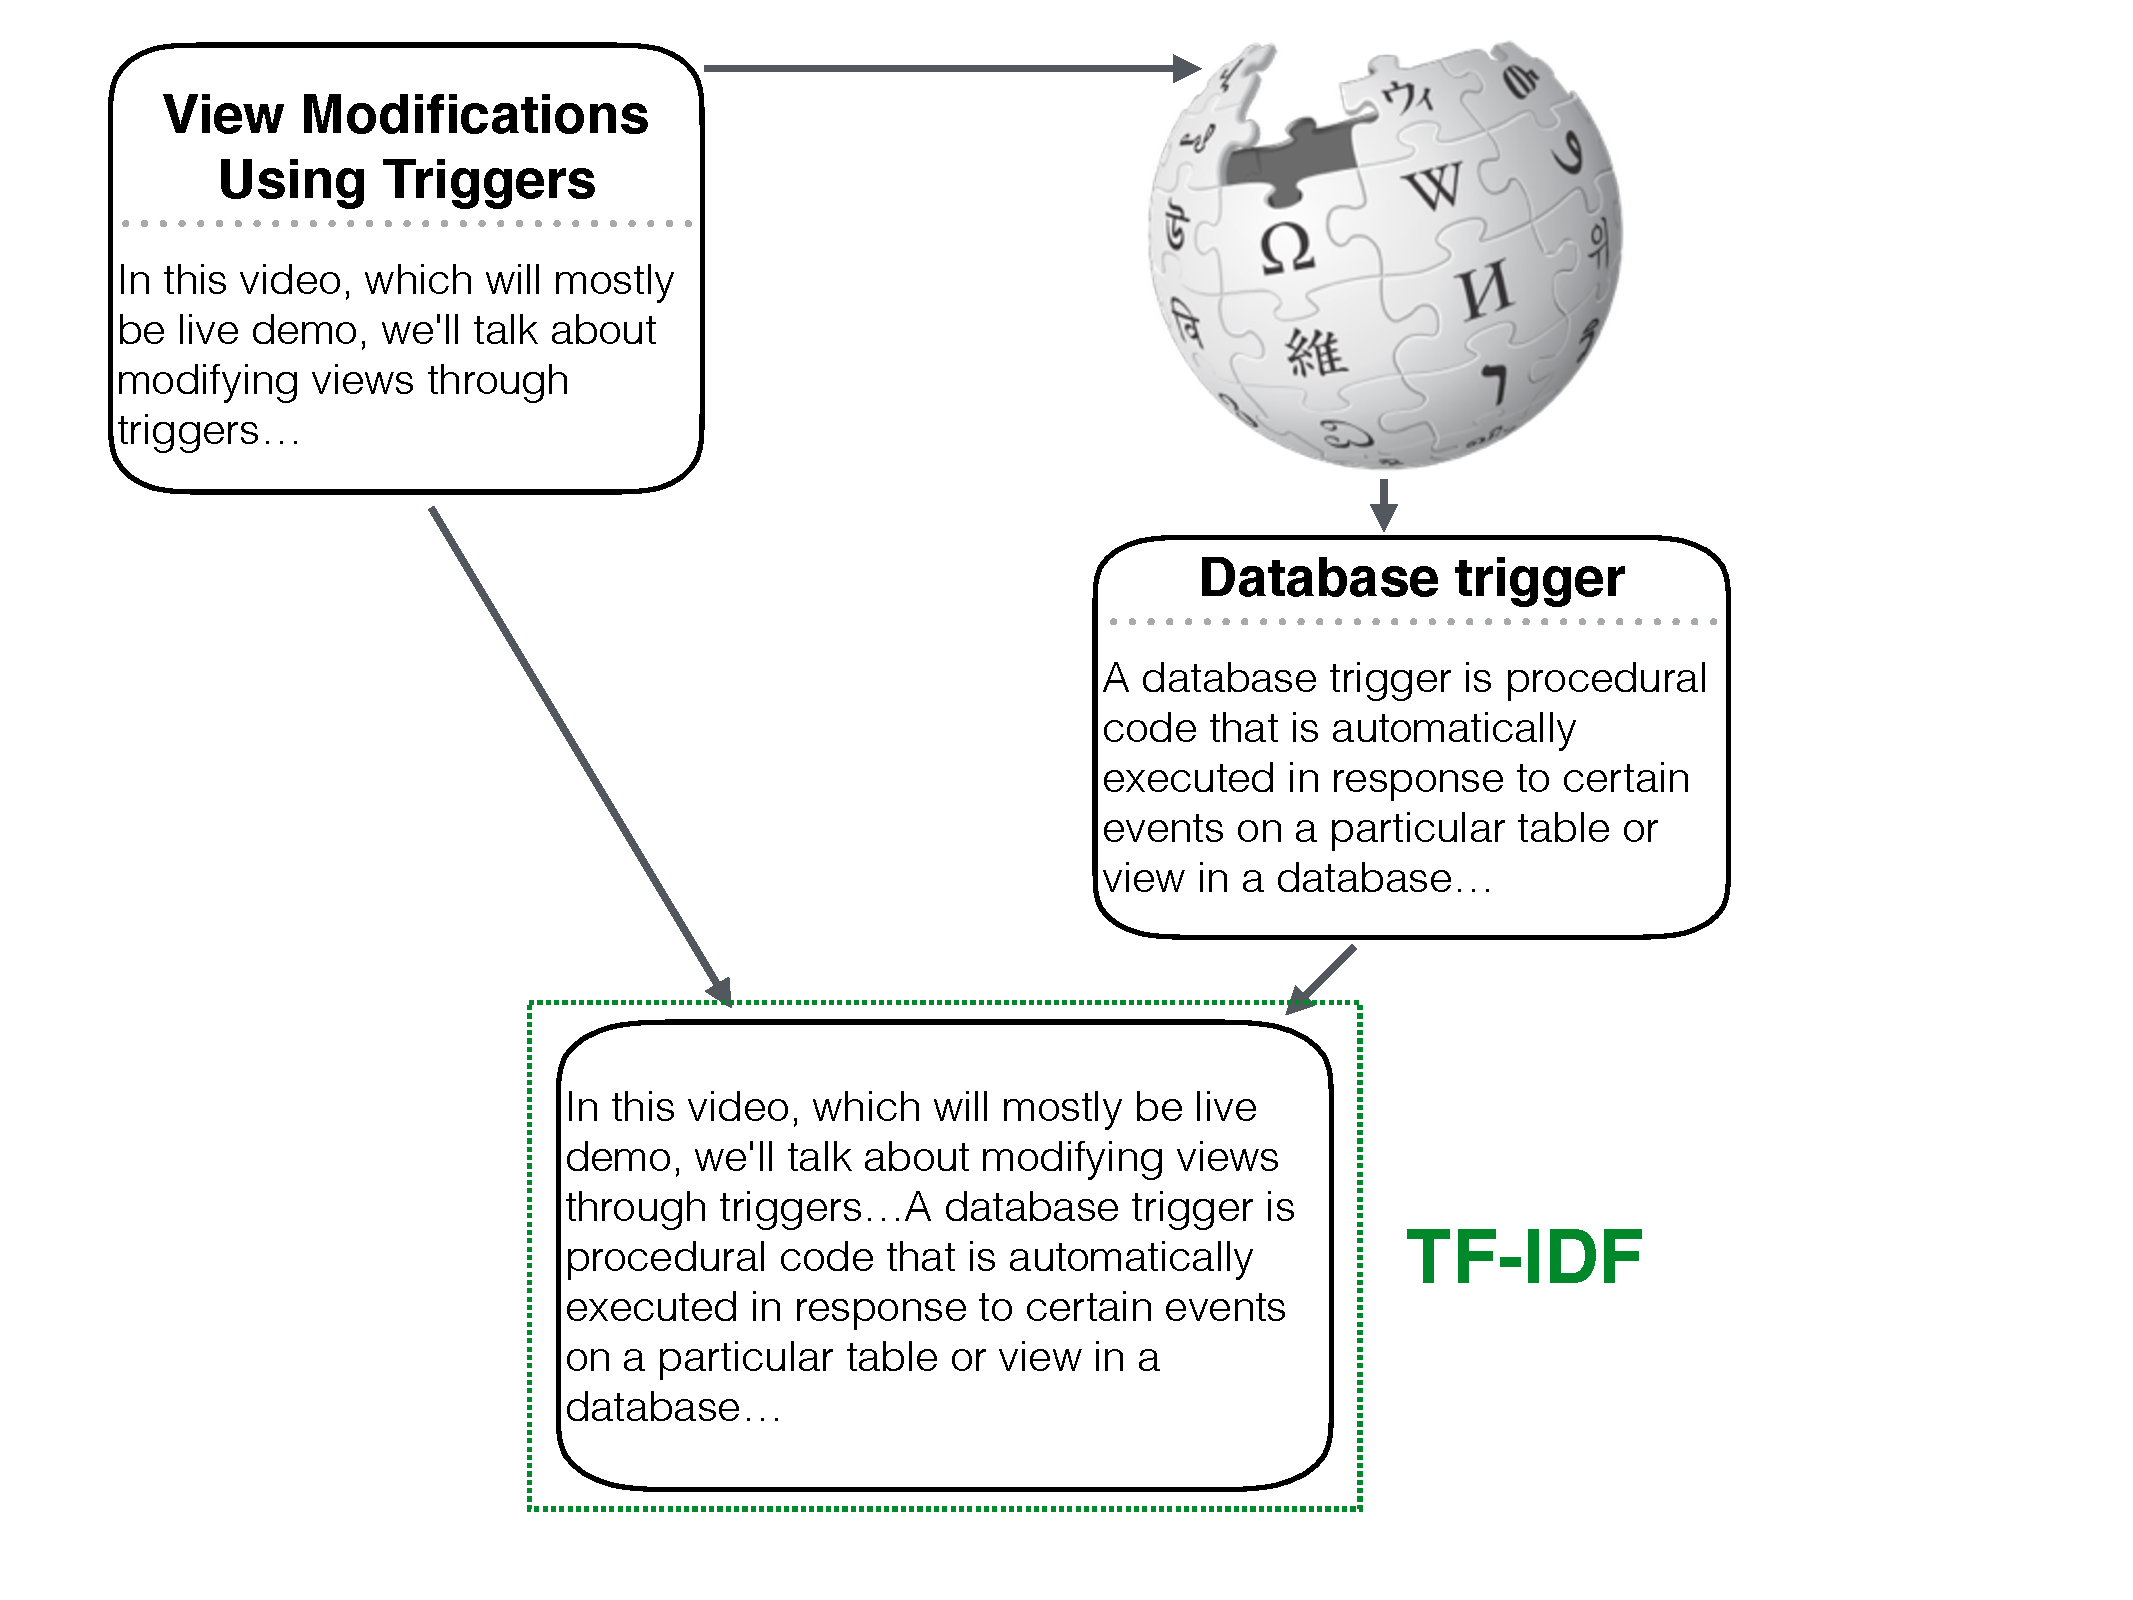
\includegraphics[width=\textwidth]{document_boosting.pdf}
\end{figure}

\subsubsection{Boosting Phrases}

This algorithm first creates a list of candidate keywords using adjective-noun phrases. Then, the candidates are ranked by their TF-IDF score summed over all Wikipedia documents. That is, for a phrase $p$, we define its term frequency $TF_w(p)$ as
\begin{equation*}
TF_w(p) \coloneqq \log\left(\text{number of times } p \text{ appears on Wikipedia}\right)
\end{equation*}state
and its inverse document frequency $IDF_w(p, W)$ for a phrase $p$ and Wikipedia article collection $W$ as
\begin{equation*}
IDF_w(p, W) \coloneqq \log\left(\frac{|W|}{\text{number of documents in } W \text{ with } p} + 1\right)
\end{equation*}
and finally $TF\text{-}IDF_w(p, W)$ is defined as
\begin{equation*}
TF\text{-}IDF_w(p, W) \coloneqq TF_w(p) \cdot IDF_w(p, W)
\end{equation*}

Next, this global candidate ranking is combined with the basic TF-IDF approach described in section \ref{sec:tfidf}. First, we create a normalized Wikipedia candidate ranking
\begin{equation*}
TF\text{-}IDF_{w-norm}(p, W) \coloneqq \frac{TF\text{-}IDF_w(p, W)}{\sum_{p'} TF\text{-}IDF_w(p', W)}
\end{equation*}
and normalized lecture collection ranking
\begin{equation*}
TF\text{-}IDF_{norm}(p, l, L) \coloneqq \frac{TF\text{-}IDF(p, l, L)}{\sum_{p'} TF\text{-}IDF(p', l, L)}
\end{equation*}
Then, we combine the two normalized rankings to form a final score
\begin{multline*}
TF\text{-}IDF_{combined}(p, l, L, W) \coloneqq \\ \eta TF\text{-}IDF_{w-norm}(p, W) + TF\text{-}IDF_{norm}(p, l, L)
\end{multline*}
where $\eta$ is used to determine the weight between Wikipedia scores and lecture scores. We found that a value of $\eta = 2$, meaning the Wikipedia ranking is weighted twice as much, seemed to work well in practice, and report those results.

We also experimented with only boosting phrases that were at least two words, based on the intution that longer phrases are often meaningful, but appear infrequently and therefore given low scores by TF-IDF. This is called ``Phrase Boosting N-Grams'' in Figure \ref{fig:main_result}, and can be thought of as multiplying $TF_w(p)$ by 0 if $p$ is not at least two tokens:
\begin{equation*}
TF_{w-ngram}(p) \coloneqq TF_w(p) \cdot \mathbf{1}\left\{p \text{ is at least two tokens}\right\}
\end{equation*}

A few subtleties deserve further description. First, in our naive TF-IDF approach, a score is calculated for each lecure $l$ and phrase $p$, while in our Wikipedia calculation a score is only calculated for each $p$. This is because in this algorithm we are not interested in keywords for every Wikipedia document, only in getting a global sense of the importance of a phrase. This is equivalent to summing over all Wikipedia documents $d \in W$
\begin{equation*}
TF_w(p) = \log \left(\sum_{d \in W} \text{number of times } p \text{ appears in } d\right)
\end{equation*}

Second, we take logarithm of the phrase count in the Wikipedia ranking. This seems to produce better empirical results.

\begin{figure}[!h]
\caption{The Phrase Boosting algorithm runs TF-IDF over the entirety of Wikipedia and then combines the global ranking with a local ranking for a document.}
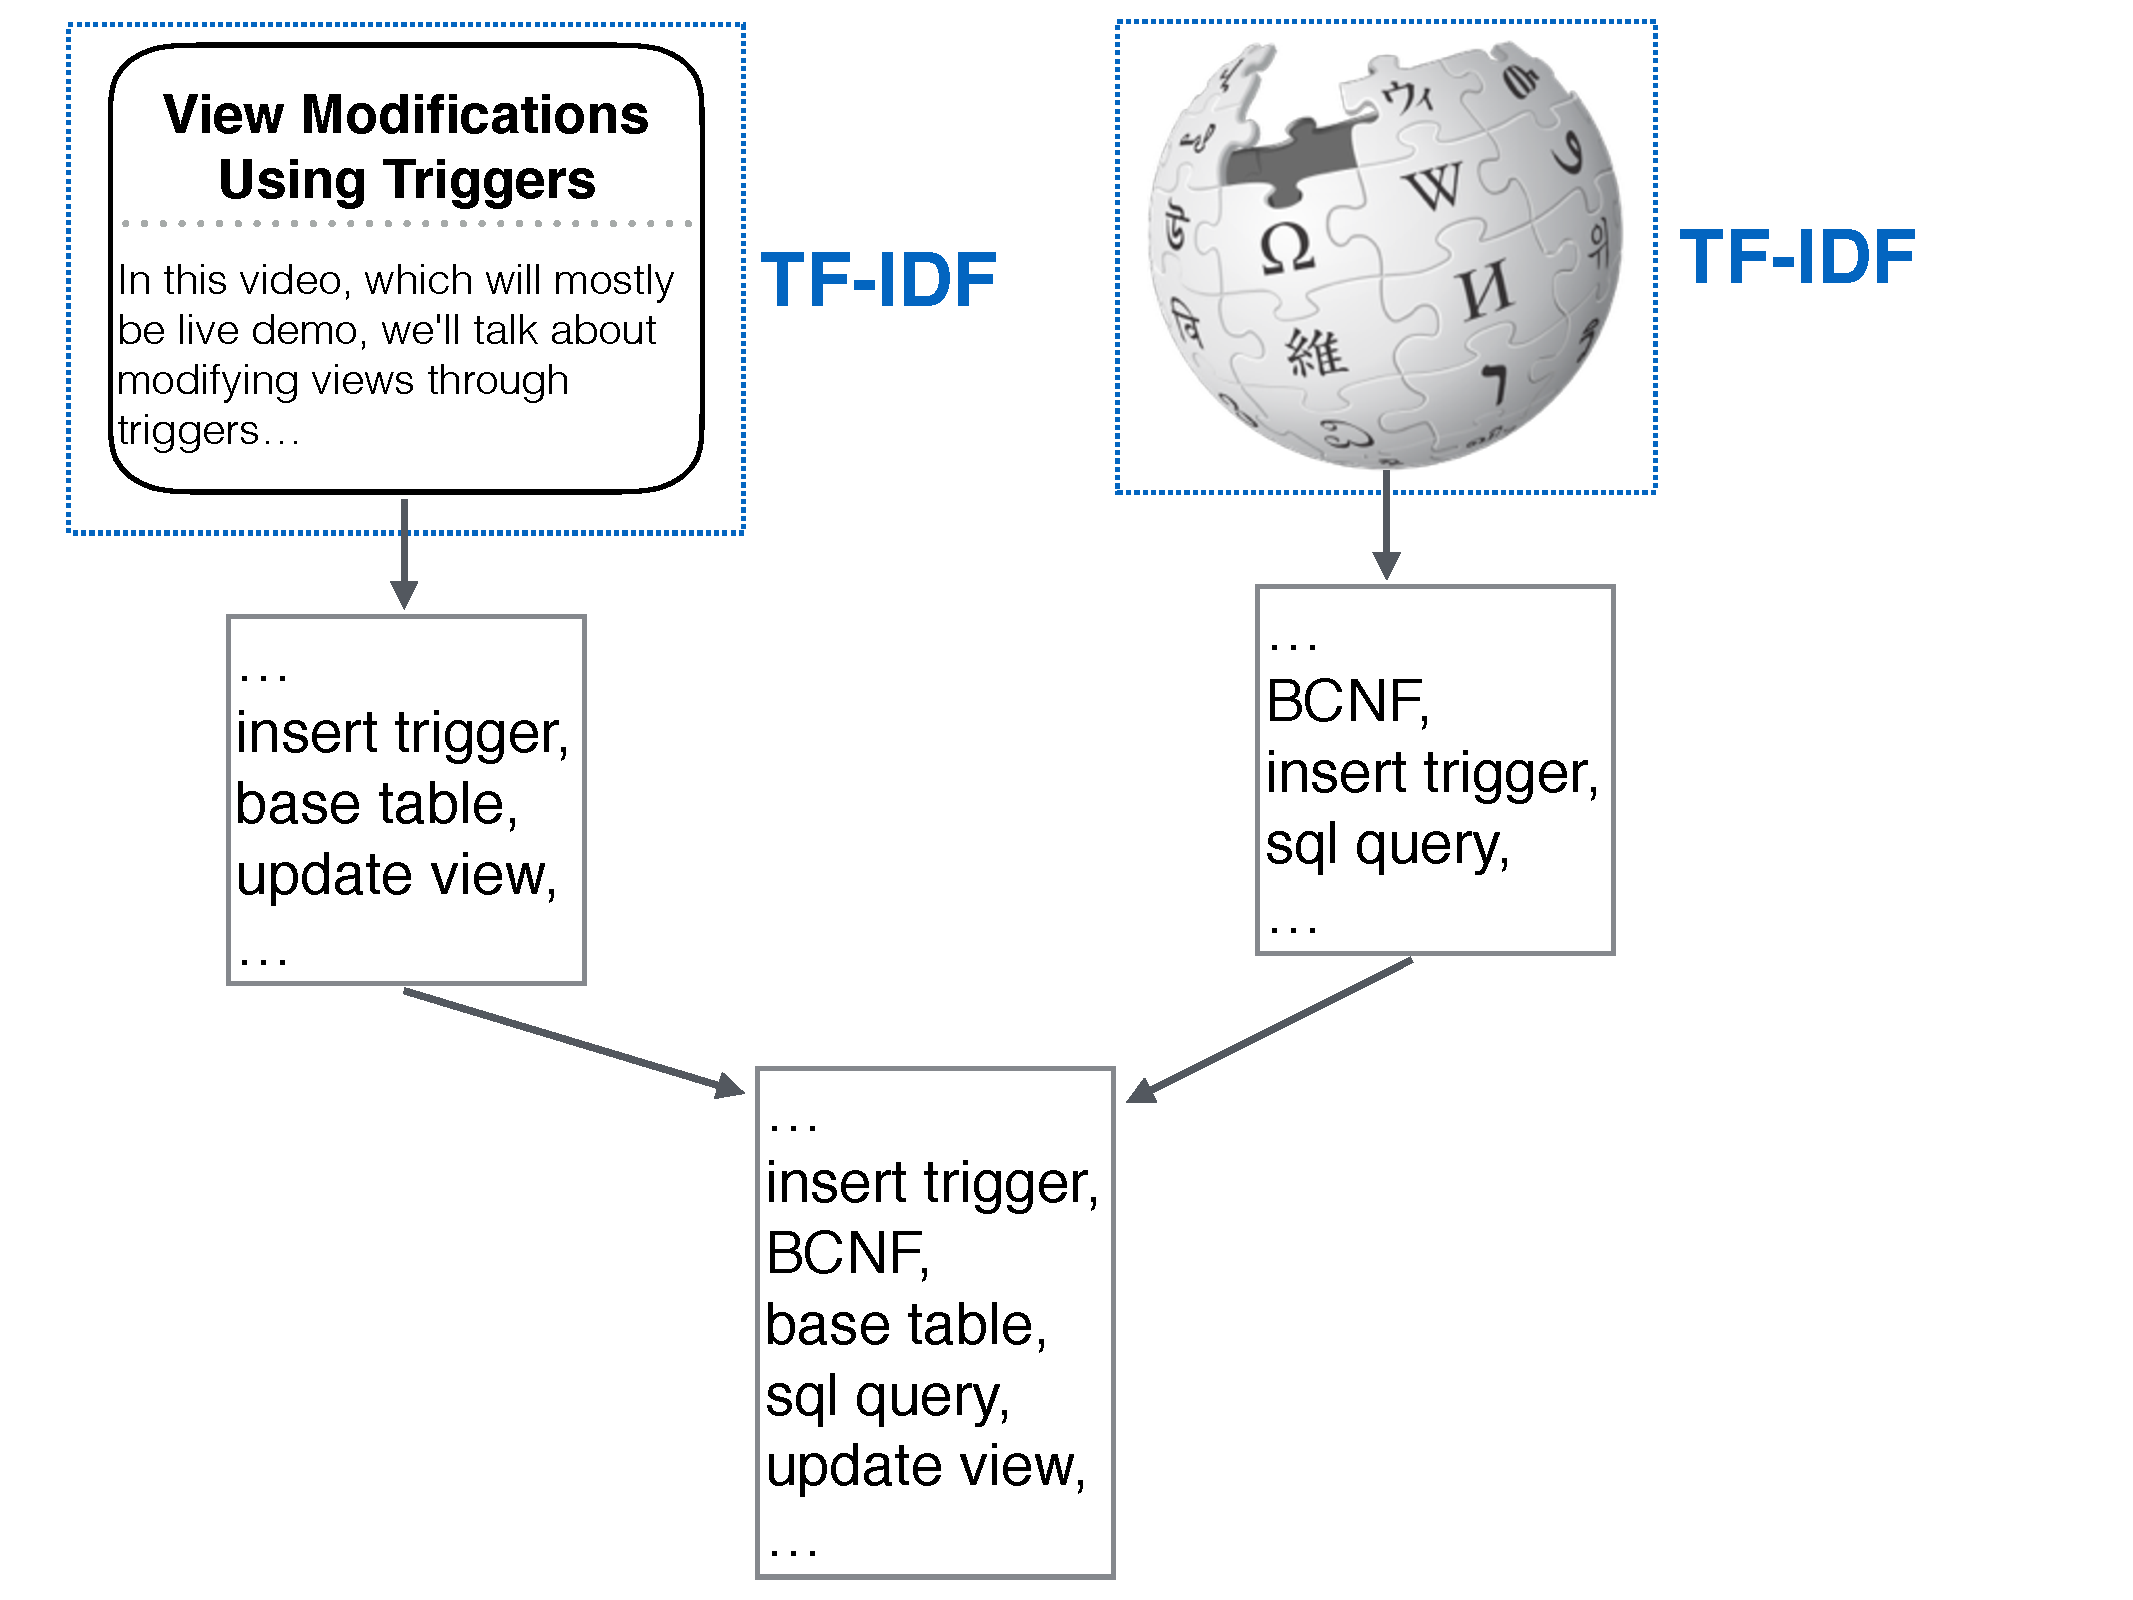
\includegraphics[width=\textwidth]{phrase_boosting.pdf}
\end{figure}
